\section{Motivation and Goals}

The estimation of the volume of a convex shape in $n$ dimensions, is a long standing problem. Exactly calculating the volume of an arbitrary convex polytope is known to be \#P-hard~\cite{Dyer88}, but it has been shown by many authors~\cite{Dyer95, Kannan97, Lovasz03}
that arbitrarily good estimates can be acquired by testing whether a polynomially bounded number of points fall within the shape. The order of this polynomial has been chipped away incrementally over many years until the most recent papers have successfully bounded the number of oracle queries to be within $O^{*}(n^4)$ and $O^{*}(n^5)$ respectively, stating that this brings the methods within the realms of a parctical implementation. Exact methods of volume computation exist and have been tested, but their scaling is measured in terms of the number of vertices and facets of the shape, not on the number of dimensions in which the shape exists. 

Our problem will be as follows. We will be given an inclusion oracle for $K$ which, on input of some point $\bm{x}$, will return either $\top$ if $\bm{x} \in K$ or $\bot$ otherwise. We also have the guarantee that $K$ is contained within a ball of known radius $R$, and that $K$ contains the unit ball. These guarantees are necessary, else we find ourselves in a situation where we may never even find the shape. We wish to construct an algorithm which, given such an oracle and an error measure $\varepsilon$, will, with high probability, return a value $v$ satisfying

$$
(1-\varepsilon)\vol(K) \leqslant v \leqslant (1+\varepsilon)\vol(K)
$$

In this study, we will test the various features of the $O^{*}(n^5)$ volume algorithm~\cite{Kannan97} by implementing a version of it in ANSI C, using various statistical methods to estimate good values for relevant parameters, and finally compare its overall execution time to a hybrid method of exact volume computation~\cite{Bueler98}. We will deliberately take a practical, intuitive approach to the data, with an aim to discuss the practicalities of these algorithms We will find that the theoretical upper bounds on most parameters are very loose indeed, and that in practice far smaller values are sufficient, resulting in significant savings on real-world execution time, however the assumption of a fast oracle proves difficult to handle, and when more detailed information about the shape is available, an exact method is still faster if the shape is simple and the number of dimensions is reasonably low. We will then discuss various subsidiary points in the appendices.

\section{Preliminaries}
\subsection{Notation}

The speed of a volume estimation algorithm is usually measured using $O^{*}$ notation, which differs from $O$ notation in that poly-logarithmic factors and factors in terms of an accuracy parameter are suppressed. This has both benefits and drawbacks. The scaling of a poly-logarithmic factor is so small that we can justifiably neglect it for most exponents, and usually we do not scale the error parameter with the number of dimensions, however hiding this sort of information makes the actual practicalities of the algorithm harder to discern. An $O^{*}(n^4)$ algorithm may seem better than an $O^{*}(n^5)$, but due to hidden scaling with error parameters and logarithmic factors, may be slower in practice. $O^{*}$ notation is a useful tool, but is not a panacea.

We will denote the volume, sometimes referred to as content~\cite{mathworld_content}, of some $n$-dimensional shape, $K$, by $\vol_n(K)$. Where a shape may exist in any number of dimensions, we will use $\vol_n$ to denote the volume of the $n$-dimensional version of that shape. Where the number of dimensions does not vary throughout an equation, we will neglect the $n$. $n$-dimensional vectors will be indexed from $1$ to $n$, with all vectors written in bold font, as in ${\bm x} = (x_1, x_2, ..., x_n)$. We will use $||\bm{x}||$ to denote the standard euclidian norm.

The notions of an $n$-ball~\cite{mathworld_ball} and an $n$-sphere~\cite{mathworld_sphere} are often subject to some confusing notation. Usually, an $n$-ball of radius $R$ is the set of points $\{{\bm x} \in \arr^n  \;\; | \;\; ||\bm{x}|| < R \}$, with the author's choice of strict or non-strict inequality. An $n$-sphere of radius $R$, however, is sometimes the set of points $\{{\bm x} \in \arr^{n+1}  \;\; | \;\; ||\bm{x}|| = R \}$, and sometimes the set of points $\{{\bm x} \in \arr^{n}  \;\; | \;\; ||\bm{x}|| = R \}$ -- note the differing dimensions. Usually, the former is used, since a sphere always refers to a surface, and an $n$-dimensional surface consists of points existing in $\arr^{n+1}$; the surface of a real-world billiard ball is a 2-dimensional surface in 3-dimensional space, so a billiard ball is a 3-ball bounded by the 2-sphere. In an attempt to avoid as much confusion on the matter as possible, however, we will avoid the term ``sphere" where possible in this report, and instead refer to the completely unambiguous notion of ``the surface of an $n$-ball".

\subsection{Shapes}

We will call any continuous subset of $\arr^{n}$ a shape. A convex shape, $K$, is one which satisfies
$$
\forall \bm{u}, \bm{v} \in K, \lambda \in [0,1] \quad (\lambda \bm{u} + (1-\lambda) \bm{v}) \in K
$$
Such a combination of points is known as a convex combination. More intuitively, we say that $K$ is convex if any straight line segment between any two points in $K$ lies entirely within $K$. $K$'s boundary does not ``bow inwards".

We will denote by $B$ the unit ball, that is $B= \{\bm{x} \in \arr^n \st ||\bm{x}|| \leqslant 1\}$, and abuse notation slightly by donoting the ball of radius $R$ by $RB$. The ball of radius $RB$ is trivially the largest convex shape that will fit within the ball of radius $RB$. Its volume is tractable~\cite{mathworld_ball}:
$$
\vol_n(RB) = \frac{\pi^{\frac{n}{2}}}{\Gamma(\frac{n}{2}+1)}R^n
$$
Where $\pi \approxeq 3.14$ denotes the circle constant, and $\Gamma(z) = \int^\infty_0 t^{z-1}e^{-t} dt$ is Euler's gamma function, computable in closed form for integers and half-integers.

The convex hull of a set of points, defined with $h(P)$, is precisely the set of points
$$
\bm{x} \in h(P) \iff \exists \bm{u}_1, \bm{u}_2,...,\bm{u}_k \in P, \lambda_1, \lambda_2, ..., \lambda_k  \in [0,1] \st \bm{x} = \sum^{k}_{i=1} \lambda_i \bm{u}_i \wedge \sum^{k}_{i=1} \lambda_i = 1
$$
Less formally, the convex hull of a set of points is the result of wrapping an elastic band around them and letting it snap tightly around them. Note that the set of points need not be finite or even discrete - we can take the convex hull of any arbitrary set of subsets of $\arr^n$. All convex hulls are convex.

We will define the $n$-dimensional ice cream of radius $R$, $RI$ as the convex hull of $B$ and the point $(R,0,0,...0)$. Figure~\ref{fig_ice_cream} should make the logic behind this name reasonably clear. The n-dimensional ice cream is important for this study because it is the smallest possible convex shape which contains $B$ and is tightly contained within $RB$. It will represent a potentially pathological case for our estimation algorithms, however as the disjoint union of a capless ball and an $n$-dimensional cone, its volume, whilst non-trivial, is calculable in terms of the volume of an $n$-ball. The details can be found in Appendix~\ref{app_ice_cream}.
$$
\vol_n(RI) = \frac{R-h}{n} \vol_{n-1}(rB) + \vol_n(B) - \left(\frac{1}{2}\vol_n(rB) I_{\frac{2rh-h^2}{r^2}}\left(\frac{n+1}{2}, \frac{1}{2}\right)\right)
$$
Where $h = \frac{1}{R}$, $r = \sqrt{1-\frac{1}{R^2}}$ and $I_x(a,b)$ is the incomplete $\beta$ function, defined thus:
$$
I_x(a,b) = \frac{\int^x_0 t^{a-1}(1-t)^{b-1}dt}{\int^1_0 t^{a-1}(1-t)^{b-1} dt}
$$
This function is the CDF of the beta distribution, and is available in various statistical packages.

\begin{figure}
\centering
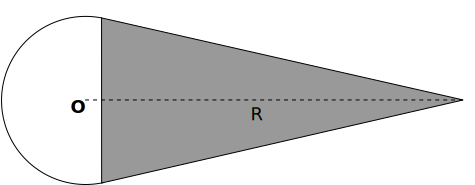
\includegraphics{./images/ice_cream_shaded.pdf}
\caption{A 2-dimensional ice-cream. The shaded part is the wafer, and the unshaded part the scoop}
\label{fig_ice_cream}
\end{figure}
\subsection{Markov Chains and Random Walks}

A Markov Chain is a triple, $(S,P,\bm{\delta})$, where $S$ is referred to as the state space, $P = (p_{st})_{s,t \in S}$ is the transition matrix and $\bm{\delta} = (\delta_s)_{s \in S}$ is the initial probability vector. A realisation of a Markov Chain is a sequence of states, $(x_i)_{i \in \nat}$ such that $\pr (x_0 = s)=\delta_s$, and $\pr(x_i = s_i | x_0 = s_0, ..., x_{i-1} = s_{i-1}) = \pr (x_i = s_i | x_{i-1} = s_{i-1})= p_{s_{i-1}s_{i}}$. We say that $\bm{\pi}$ is a stationary distribution of the Markov Chain if, given that $\bm{\delta} = \bm{\pi}$, the marginal probabilities $\pr(x_i = t) = \pi_t$ for all $i$ and $t$.  It is a standard result from probability that, if one can find a probability distribution $\bm{\pi}$ such that
$$
\forall s,t \in S, \quad \pi_s p_{st} = \pi_t p_{ts}
$$
Then $\bm{\pi}$ is the stationary distribution for the chain. It should be reasonably obvious that, if $p_{ij} = p_{ji}$ for all pairs of states, then $\bm{\pi}$ is a constant. If a stationary distribution exists for a chain, then, regardless of $\bm{\delta}$, $\lim_{i-> \infty} \pr {x_i = s} = \pi_s$.

A random walk through a shape is a Markov Chain whose state space approximates the interior of a shape. We will use a random walk to sample uniformly at random from the inerior of a shape. By selecting a walk that satisfies $p_{ij} = p_{ji}$, we can can trace some number of steps from this walk, and return the state after this many steps. The walk we use will be the Hit and Run Walk~\cite{Lovasz03a}, which has been shown both theoretically and in practice to rapidly approach its stationary distribution, requiring a very small number of steps to produce good randomness. For a walk in the interior of $K$, starting at $\bm{x}_0$, the Hit and Run walk selects a line uniformly at random passing through $\bm{x}_0$ and contained entirely within $K$, then moves to a point uniformly distributed along this line. The number of times this needs to be repeated before a point becomes near-uniformly distributed in $K$ depends on $n$, and this will be discussed in section \ref{sec_mix}

Selecting the line through $\bm{x}_0$ can be accomplished by standard hyperspherical point picking~\cite{mathworld_picking} followed by a binary search. We sample $n$ independent standard normal random variables to pick a random point $\bm{u}$ on the surface of the $n$-dimensional unit ball, and define the line $\{\bm{x} | \bm{x} = \bm{x}_0 + \lambda \bm{u}, \lambda \in \arr \}$. Since we know that $K$ is contained within the ball of radius $R$, we know that $\bm{x}_0 + 2R\bm{u} \notin K$, and so can perform a bidirectional binary search to find $\overline{\lambda}$ and $\underline{\lambda}$ such that $\{\bm{x} | \bm{x} = \bm{x}_0 + \lambda \bm{u}, \lambda \in [\underline{\lambda}, \overline{\lambda}] \}$ is tightly contained within $K$. Selecting a $U(\underline{\lambda}, \overline{\lambda})$ random variable will then let us move to a uniformly random point on this line. Algorithm \ref{alg_samp} specifies this process. Since $R \in O(\sqrt{n})$, the two while loops form a binary search on a set of bins in $O(\log(\frac{2R}{\theta})) = O^{*}(1)$ time. 

\begin{algorithm}
\SetAlgoLined
\SetKwInOut{Input}{input}
\SetKwInOut{Output}{output}

\caption{An Algorithm for Generating an Approximately Uniformly Distributed Random Point in a Convex Shape}\label{alg_samp}
\Input{$K$, a convex shape for which a membership oracle can be implemented easily, $n$, the number of dimensions in which $K$ exists, $R$, the radius of $K$, $n_s$, the number of steps to take before returning, and $\theta$, an accuracy parameter}
\Output{$\bm p$, a point in $K$ randomly distributed to be near uniform on $K$}

\Begin{
	${\bm p} <- 0$ \\
	\For{$i <- 1$ \KwTo $n_s$}{
		$\bm{u} <-$ random\_direction \\
		$\overline{\lambda}' <- {\bm p} + 2R \bm{u}$ \\
		$\overline{\lambda}  <- 0$ \\
		$\underline{\lambda}' <- {\bm p} - 2R \bm{u}$ \\
		$\underline{\lambda}  <- 0$ \\
		\While{$\overline{\lambda}' - \overline{\lambda} > \theta$}{
			\uIf{${\bm p} + \frac{\overline{\lambda} + \overline{\lambda}'}{2}\bm{u} \in K$}{
				$\overline{\lambda}  <- \frac{\overline{\lambda} + \overline{\lambda}'}{2}$
			}\Else{
				$\overline{\lambda}' <- \frac{\overline{\lambda} + \overline{\lambda}'}{2}$
			}
		}
		\While{$\underline{\lambda}' - \underline{\lambda} > \theta$}{
			\uIf{${\bm p} + \frac{\underline{\lambda} + \underline{\lambda}'}{2}\bm{u} \in K$}{
				$\underline{\lambda}  <- \frac{\underline{\lambda} + \underline{\lambda}'}{2}$
			}\Else{
				$\underline{\lambda}' <- \frac{\underline{\lambda} + \underline{\lambda}'}{2}$
			}
		}
		$\lambda <-$uniform$(\underline{\lambda}, \overline{\lambda})$\\
		${\bm p} <- {\bm p} + \lambda \bm{u}$
	}
	\KwRet $\bm p$
}
\end{algorithm}

In the implementation, uniform random numbers are selected via the Mersenne Twister~\cite{Matsumoto98}, and normally distributed random numbers are selected with the Ziggurat algorithm~\cite{Marsaglia00, Burkardt07}. These two methods are known to generate high quality random numbers quickly.

\subsection{The Volume Estimation Algorithm}

The algorithm will follow Kannan, Ravi, Lov\'{a}sz and Simonovits~\cite{Kannan97} with a few minor differences. Rather than generating random points using the ball walk, we generate points with Hit and Run. Rather than using $2$ as the base for our exponents, we use $e$.

To estimate the volume of some shape, $K$, we choose a sequence of shapes, $K_0 \subseteq K_1 \subseteq ... \subseteq K_p$, such that volume $\vol (K_0)$ can be computed easily, $K_p = K$, and we can estimate the ratios $\frac{\vol(K_{i+1})}{\vol(K_i)}$ easily. Given good estimates for all of these values, we have that
$$
\vol(K) = \vol(K_0) \frac{\vol(K_1)}{\vol(K_0)} \frac{\vol(K_2)}{\vol(K_1)} \frac{\vol(K_3)}{\vol(K_2)} \, ... \, \frac{\vol(K_p)}{\vol(K_{p-1})}
$$
For this algorithm, the shapes $K_i = (e^{i/n}B) \cap K$ for $i = 0, ..., n \log (R)$ are used. Since $B \subseteq K \subseteq RB$, this satisfies our first two conditions. We can then estimate the ratios by sampling uniformly at random from $K_i$ and counting the number of points which fall into $K_{i-1}$. Modifying an oracle that samples from $K$ such that it samples from $K_i$ is fairly easy, given ${\bm x}$ we return $\top$ iff $||\bm{x}||_2 < e^{i/n}$ and ${\bm x} \in K$. The ratio of volumes can be estimated as the fraction of uniformly generated random points in $K_i$ that fall into $K_{i-1}$. Algorithm~\ref{alg_vol} specifies this in pseudocode.

\begin{algorithm}
\SetAlgoLined
\SetKwInOut{Input}{input}
\SetKwInOut{Output}{output}

\caption{An Algorithm for Estimating the Volume of a Convex Shape}\label{alg_vol}
\Input{$K$, a convex shape for which a membership oracle can be implemented easily, $n$, the number of dimensions in which $K$ exists, $R$, the radius of $K$, and $n_p$, a number of points to use per thread}
\Output{$v$, an estimate of $vol(K)$}

\Begin{
	$n_s <- \lfloor n \ln (R) + 1 \rfloor$ \\
	$v <-\vol_n(B)$ \\
	$K_0 <- B$
	\For{$i <- 1$ \KwTo $n_s$}{
		$K_i <- e^\frac{i}{n}B \cap K$ \\
		$n_{in} <- 0$
		\For{$j <- 1$ \KwTo $n_p$}{
			$\bm{p} <-$ generate\_point$(K_i)$ \\
			\If{$\bm{p} \in K_{i-1}$}{
				$n_{in} <- n_{in} + 1$
			}
		}
		$v <- \frac{n_s v}{n_{in}}$
	}
	\KwRet $v$
}
\end{algorithm}

\subsection{Neglected Details}

This field is very well researched, and not every part of this research can be accounted for in this study.

Firstly, when sampling a point, the sampling algorithm is actually capable of starting from any arbitrary location. The line ${\bm p} <- 0$ from algorithm \ref{alg_samp} can instead be a previously generated point, passed as a parameter, to be perturbed by the random walk. The algorithms in the literature tend to use the previously generated point as a starting point, thus providing a ``warm start" to the random walk. Preliminary experiments showed that this produced random numbers of lower quality than starting from $0$ every time.

The literature assumes that, if $K \subseteq RB$, then $R \in O^{*}(\sqrt{n})$. If this is not the case, then it is fairly easy to transform space such that it is, for some predetermined constant factors hidden by the $O$ notation. In this study, we will ignore this by simply generating shapes for which $R = \sqrt{n}$ in every case. This transformation also includes a translation such that the centre of $K$'s mass is at the origin. This provides a useful technical tool to make the analysis easier, but is not necessary for the algorithms to be correct. Similarly, we neglect the step of adjusting the size of the shape such that the covariance matrix of its uniform distribution is the identity.

A much faster algorithm than the one used does exist at this time~\cite{Lovasz03}. This algorithm claims an asymptotic complexity of $O^{*}(n^4)$, but is significantly harder to implement. In the interest of getting usable results out in a reasonable timeframe, this paper has not been used, however some of the techniques within it, such as the Hit and Run walk, have been adapted for this study.